\appendix
\section{Diagram voor Diagnose van Tremoren}
\label{appendix:diagnose}

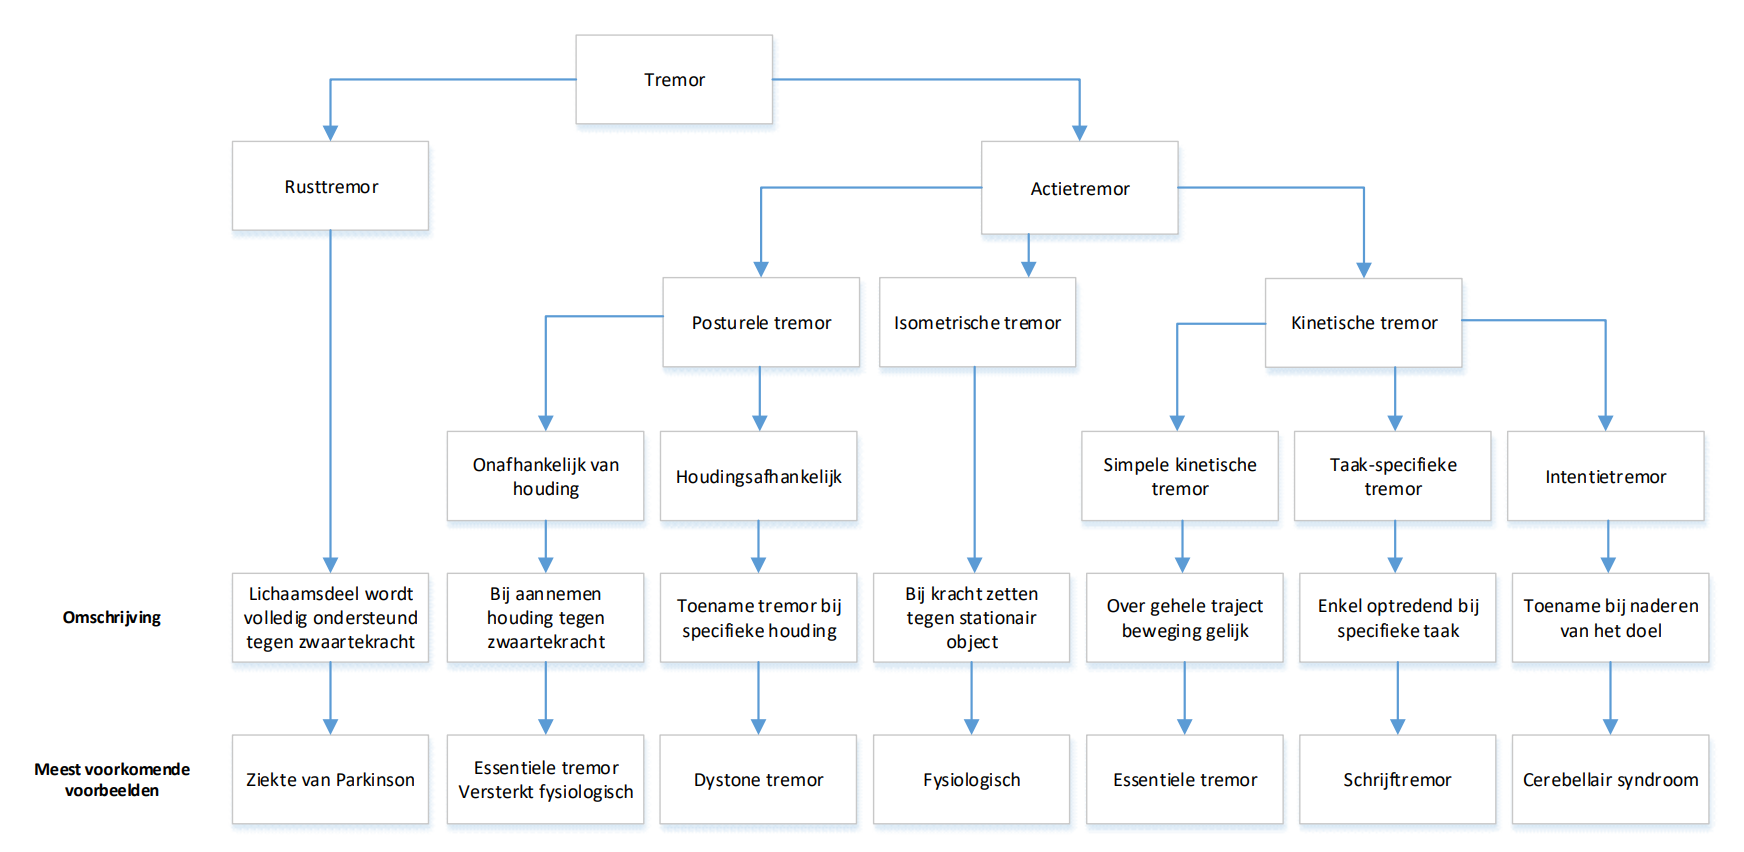
\includegraphics[width=\textwidth]{graphics/graph-tremor-diagnosis.png}

\section{Interview Tremoren en Tremor Registratie}

Tremoren komen het vaakst voor bij Essentiële Tremor en Parkinsons.
Ongeveer 30\% van de gevallen betreft Parkinsons.
Het verschil tussen de twee aandoeningen is dat ET vooral bij actie voorkomt.
Er zijn echter vele variaties van tremoren, welke tremor, is onder andere door de frequentie te meten.

De registratie wordt in het geval van het Admiraal de Ruyter Ziekenhuis gedaan in Vlissingen.
Om van tevoren een inschatting te kunnen maken, kan er gebruik worden gemaakt van apps die trillingen kunnen meten.
Er is wel medicatie beschikbaar voor de aandoening, maar deze zijn niet oorspronkelijk bedoeld voor ET.

Bij Parkinsons valt het resultaat van deze medicatie vaak tegen. Er is dus een vraag naar alternatieven.
Een mogelijke alternatief is DBS (Deep Brain Stimulation). Een ingrijpende, maar effectieve behandeling.
UltraSound is een alternatief dat vooral in Japan wordt gebruikt. Het belooft veel,
maar is nog niet effectief genoeg voor realisatie.

DBS is relatief functioneel en veilig. De behandelingen worden vooral gedaan in Tilburg, Leiden,
Maastricht, Groningen en Amsterdam. Het bestaat 25 jaar en er is experimentele AI voor het lezen en sturen hiervan.

Het registreren van een tremor gebeurd vooral met een EMG (Elektromyogram). Dit brengt spieractiviteit in kaart.
Er zijn polshorloges beschikbaar die dit kunnen meten. 
Deze worden in de praktijk vooral gebruikt voor het meten van stijfheid en overbewegelijkheid.